% Options for packages loaded elsewhere
\PassOptionsToPackage{unicode}{hyperref}
\PassOptionsToPackage{hyphens}{url}
\PassOptionsToPackage{dvipsnames,svgnames,x11names}{xcolor}
%
\documentclass[
  letterpaper,
  DIV=11,
  numbers=noendperiod]{scrartcl}

\usepackage{amsmath,amssymb}
\usepackage{iftex}
\ifPDFTeX
  \usepackage[T1]{fontenc}
  \usepackage[utf8]{inputenc}
  \usepackage{textcomp} % provide euro and other symbols
\else % if luatex or xetex
  \usepackage{unicode-math}
  \defaultfontfeatures{Scale=MatchLowercase}
  \defaultfontfeatures[\rmfamily]{Ligatures=TeX,Scale=1}
\fi
\usepackage{lmodern}
\ifPDFTeX\else  
    % xetex/luatex font selection
    \setmainfont[]{Times New Roman}
\fi
% Use upquote if available, for straight quotes in verbatim environments
\IfFileExists{upquote.sty}{\usepackage{upquote}}{}
\IfFileExists{microtype.sty}{% use microtype if available
  \usepackage[]{microtype}
  \UseMicrotypeSet[protrusion]{basicmath} % disable protrusion for tt fonts
}{}
\makeatletter
\@ifundefined{KOMAClassName}{% if non-KOMA class
  \IfFileExists{parskip.sty}{%
    \usepackage{parskip}
  }{% else
    \setlength{\parindent}{0pt}
    \setlength{\parskip}{6pt plus 2pt minus 1pt}}
}{% if KOMA class
  \KOMAoptions{parskip=half}}
\makeatother
\usepackage{xcolor}
\usepackage[lmargin=2cm,rmargin=2cm,tmargin=1.5cm]{geometry}
\setlength{\emergencystretch}{3em} % prevent overfull lines
\setcounter{secnumdepth}{5}
% Make \paragraph and \subparagraph free-standing
\makeatletter
\ifx\paragraph\undefined\else
  \let\oldparagraph\paragraph
  \renewcommand{\paragraph}{
    \@ifstar
      \xxxParagraphStar
      \xxxParagraphNoStar
  }
  \newcommand{\xxxParagraphStar}[1]{\oldparagraph*{#1}\mbox{}}
  \newcommand{\xxxParagraphNoStar}[1]{\oldparagraph{#1}\mbox{}}
\fi
\ifx\subparagraph\undefined\else
  \let\oldsubparagraph\subparagraph
  \renewcommand{\subparagraph}{
    \@ifstar
      \xxxSubParagraphStar
      \xxxSubParagraphNoStar
  }
  \newcommand{\xxxSubParagraphStar}[1]{\oldsubparagraph*{#1}\mbox{}}
  \newcommand{\xxxSubParagraphNoStar}[1]{\oldsubparagraph{#1}\mbox{}}
\fi
\makeatother

\usepackage{color}
\usepackage{fancyvrb}
\newcommand{\VerbBar}{|}
\newcommand{\VERB}{\Verb[commandchars=\\\{\}]}
\DefineVerbatimEnvironment{Highlighting}{Verbatim}{commandchars=\\\{\}}
% Add ',fontsize=\small' for more characters per line
\usepackage{framed}
\definecolor{shadecolor}{RGB}{241,243,245}
\newenvironment{Shaded}{\begin{snugshade}}{\end{snugshade}}
\newcommand{\AlertTok}[1]{\textcolor[rgb]{0.68,0.00,0.00}{#1}}
\newcommand{\AnnotationTok}[1]{\textcolor[rgb]{0.37,0.37,0.37}{#1}}
\newcommand{\AttributeTok}[1]{\textcolor[rgb]{0.40,0.45,0.13}{#1}}
\newcommand{\BaseNTok}[1]{\textcolor[rgb]{0.68,0.00,0.00}{#1}}
\newcommand{\BuiltInTok}[1]{\textcolor[rgb]{0.00,0.23,0.31}{#1}}
\newcommand{\CharTok}[1]{\textcolor[rgb]{0.13,0.47,0.30}{#1}}
\newcommand{\CommentTok}[1]{\textcolor[rgb]{0.37,0.37,0.37}{#1}}
\newcommand{\CommentVarTok}[1]{\textcolor[rgb]{0.37,0.37,0.37}{\textit{#1}}}
\newcommand{\ConstantTok}[1]{\textcolor[rgb]{0.56,0.35,0.01}{#1}}
\newcommand{\ControlFlowTok}[1]{\textcolor[rgb]{0.00,0.23,0.31}{\textbf{#1}}}
\newcommand{\DataTypeTok}[1]{\textcolor[rgb]{0.68,0.00,0.00}{#1}}
\newcommand{\DecValTok}[1]{\textcolor[rgb]{0.68,0.00,0.00}{#1}}
\newcommand{\DocumentationTok}[1]{\textcolor[rgb]{0.37,0.37,0.37}{\textit{#1}}}
\newcommand{\ErrorTok}[1]{\textcolor[rgb]{0.68,0.00,0.00}{#1}}
\newcommand{\ExtensionTok}[1]{\textcolor[rgb]{0.00,0.23,0.31}{#1}}
\newcommand{\FloatTok}[1]{\textcolor[rgb]{0.68,0.00,0.00}{#1}}
\newcommand{\FunctionTok}[1]{\textcolor[rgb]{0.28,0.35,0.67}{#1}}
\newcommand{\ImportTok}[1]{\textcolor[rgb]{0.00,0.46,0.62}{#1}}
\newcommand{\InformationTok}[1]{\textcolor[rgb]{0.37,0.37,0.37}{#1}}
\newcommand{\KeywordTok}[1]{\textcolor[rgb]{0.00,0.23,0.31}{\textbf{#1}}}
\newcommand{\NormalTok}[1]{\textcolor[rgb]{0.00,0.23,0.31}{#1}}
\newcommand{\OperatorTok}[1]{\textcolor[rgb]{0.37,0.37,0.37}{#1}}
\newcommand{\OtherTok}[1]{\textcolor[rgb]{0.00,0.23,0.31}{#1}}
\newcommand{\PreprocessorTok}[1]{\textcolor[rgb]{0.68,0.00,0.00}{#1}}
\newcommand{\RegionMarkerTok}[1]{\textcolor[rgb]{0.00,0.23,0.31}{#1}}
\newcommand{\SpecialCharTok}[1]{\textcolor[rgb]{0.37,0.37,0.37}{#1}}
\newcommand{\SpecialStringTok}[1]{\textcolor[rgb]{0.13,0.47,0.30}{#1}}
\newcommand{\StringTok}[1]{\textcolor[rgb]{0.13,0.47,0.30}{#1}}
\newcommand{\VariableTok}[1]{\textcolor[rgb]{0.07,0.07,0.07}{#1}}
\newcommand{\VerbatimStringTok}[1]{\textcolor[rgb]{0.13,0.47,0.30}{#1}}
\newcommand{\WarningTok}[1]{\textcolor[rgb]{0.37,0.37,0.37}{\textit{#1}}}

\providecommand{\tightlist}{%
  \setlength{\itemsep}{0pt}\setlength{\parskip}{0pt}}\usepackage{longtable,booktabs,array}
\usepackage{calc} % for calculating minipage widths
% Correct order of tables after \paragraph or \subparagraph
\usepackage{etoolbox}
\makeatletter
\patchcmd\longtable{\par}{\if@noskipsec\mbox{}\fi\par}{}{}
\makeatother
% Allow footnotes in longtable head/foot
\IfFileExists{footnotehyper.sty}{\usepackage{footnotehyper}}{\usepackage{footnote}}
\makesavenoteenv{longtable}
\usepackage{graphicx}
\makeatletter
\def\maxwidth{\ifdim\Gin@nat@width>\linewidth\linewidth\else\Gin@nat@width\fi}
\def\maxheight{\ifdim\Gin@nat@height>\textheight\textheight\else\Gin@nat@height\fi}
\makeatother
% Scale images if necessary, so that they will not overflow the page
% margins by default, and it is still possible to overwrite the defaults
% using explicit options in \includegraphics[width, height, ...]{}
\setkeys{Gin}{width=\maxwidth,height=\maxheight,keepaspectratio}
% Set default figure placement to htbp
\makeatletter
\def\fps@figure{htbp}
\makeatother

\KOMAoption{captions}{tableheading}
\makeatletter
\@ifpackageloaded{caption}{}{\usepackage{caption}}
\AtBeginDocument{%
\ifdefined\contentsname
  \renewcommand*\contentsname{Table of contents}
\else
  \newcommand\contentsname{Table of contents}
\fi
\ifdefined\listfigurename
  \renewcommand*\listfigurename{List of Figures}
\else
  \newcommand\listfigurename{List of Figures}
\fi
\ifdefined\listtablename
  \renewcommand*\listtablename{List of Tables}
\else
  \newcommand\listtablename{List of Tables}
\fi
\ifdefined\figurename
  \renewcommand*\figurename{Figure}
\else
  \newcommand\figurename{Figure}
\fi
\ifdefined\tablename
  \renewcommand*\tablename{Table}
\else
  \newcommand\tablename{Table}
\fi
}
\@ifpackageloaded{float}{}{\usepackage{float}}
\floatstyle{ruled}
\@ifundefined{c@chapter}{\newfloat{codelisting}{h}{lop}}{\newfloat{codelisting}{h}{lop}[chapter]}
\floatname{codelisting}{Listing}
\newcommand*\listoflistings{\listof{codelisting}{List of Listings}}
\makeatother
\makeatletter
\makeatother
\makeatletter
\@ifpackageloaded{caption}{}{\usepackage{caption}}
\@ifpackageloaded{subcaption}{}{\usepackage{subcaption}}
\makeatother
\makeatletter
\@ifpackageloaded{tikz}{}{\usepackage{tikz}}
\makeatother
        \newcommand*\circled[1]{\tikz[baseline=(char.base)]{
          \node[shape=circle,draw,inner sep=1pt] (char) {{\scriptsize#1}};}}  
                  

\ifLuaTeX
  \usepackage{selnolig}  % disable illegal ligatures
\fi
\usepackage{bookmark}

\IfFileExists{xurl.sty}{\usepackage{xurl}}{} % add URL line breaks if available
\urlstyle{same} % disable monospaced font for URLs
\hypersetup{
  pdftitle={Chapter 5 Review},
  pdfauthor={Anthony Tricarico},
  colorlinks=true,
  linkcolor={blue},
  filecolor={Maroon},
  citecolor={Blue},
  urlcolor={Blue},
  pdfcreator={LaTeX via pandoc}}


\title{Chapter 5 Review}
\author{Anthony Tricarico}
\date{}

\begin{document}
\maketitle

\renewcommand*\contentsname{Table of contents}
{
\hypersetup{linkcolor=}
\setcounter{tocdepth}{3}
\tableofcontents
}

\section{Intro}\label{intro}

This is an explanation of the code used for chapter 5. This chapter of
the textbook is focused on producing our first forecasts after fitting
various models to our time series data. The models in this chapter are
meant to be simple so that we can then use them as benchmark methods for
more advanced models that will be developed in the next chapters.

Also, this review will assume that you already know and have acquired
basic familiarity with the functions explained up until the third
chapter. Note that we will not cover all the mathematical aspects
included in the book to keep these explanations simple enough, but of
course if you feel like it you can just read through the chapter to
understand what is really going on behind the scenes. Finally, if you
did not cover basic topics in probability theory and hypothesis testing
yet, this is the right moment to do so because we will use these
concepts frequently in the following sections of this review and those
concepts will be useful in the future (e.g., for your quantitative
methods class).

\section{Basic functions for Modeling and
Forecasting}\label{basic-functions-for-modeling-and-forecasting}

This section is an overview of the most important functions that we will
use to model our data and produce the first forecasts. First let's
import the library that contains the functions we will use.

\begin{Shaded}
\begin{Highlighting}[]
\FunctionTok{library}\NormalTok{(fpp3)}
\end{Highlighting}
\end{Shaded}

\begin{verbatim}
Registered S3 method overwritten by 'tsibble':
  method               from 
  as_tibble.grouped_df dplyr
\end{verbatim}

\begin{verbatim}
-- Attaching packages -------------------------------------------- fpp3 1.0.1 --
\end{verbatim}

\begin{verbatim}
v tibble      3.2.1     v tsibble     1.1.5
v dplyr       1.1.4     v tsibbledata 0.4.1
v tidyr       1.3.1     v feasts      0.4.1
v lubridate   1.9.3     v fable       0.4.1
v ggplot2     3.5.1     
\end{verbatim}

\begin{verbatim}
-- Conflicts ------------------------------------------------- fpp3_conflicts --
x lubridate::date()    masks base::date()
x dplyr::filter()      masks stats::filter()
x tsibble::intersect() masks base::intersect()
x tsibble::interval()  masks lubridate::interval()
x dplyr::lag()         masks stats::lag()
x tsibble::setdiff()   masks base::setdiff()
x tsibble::union()     masks base::union()
\end{verbatim}

\subsection{\texorpdfstring{\texttt{TSLM()}}{TSLM()}}\label{sec-tslm}

This function allows you to fit a linear model using the components of a
time series (i.e., trend or seasonality).

\phantomsection\label{annotated-cell-2}%
\begin{Shaded}
\begin{Highlighting}[]
\FunctionTok{TSLM}\NormalTok{(GDP\_per\_capita }\SpecialCharTok{\textasciitilde{}} \FunctionTok{trend}\NormalTok{()) }\hspace*{\fill}\NormalTok{\circled{1}}
\end{Highlighting}
\end{Shaded}

\begin{description}
\tightlist
\item[\circled{1}]
This is how you specify a formula, on the left of the \textasciitilde{}
there is the dependent variable and on its right stands the independent
variable (i.e., trend)
\end{description}

\begin{verbatim}
<TSLM model definition>
\end{verbatim}

In order to use this formula to fit a linear model you need to use the
\texttt{model()} function.

\subsection{\texorpdfstring{\texttt{model()}}{model()}}\label{model}

This is how you use the model function to fit a model to your data:

\phantomsection\label{annotated-cell-3}%
\begin{Shaded}
\begin{Highlighting}[]
\NormalTok{gdppc }\OtherTok{\textless{}{-}} \FunctionTok{mutate}\NormalTok{(global\_economy, }\StringTok{"GDP\_per\_capita"} \OtherTok{=}\NormalTok{ GDP }\SpecialCharTok{/}\NormalTok{ Population) }\hspace*{\fill}\NormalTok{\circled{1}}

\NormalTok{(fit }\OtherTok{\textless{}{-}} \FunctionTok{model}\NormalTok{(gdppc, }\AttributeTok{trend\_model =} \FunctionTok{TSLM}\NormalTok{(GDP\_per\_capita }\SpecialCharTok{\textasciitilde{}} \FunctionTok{trend}\NormalTok{()))) }\hspace*{\fill}\NormalTok{\circled{2}}
\end{Highlighting}
\end{Shaded}

\begin{description}
\tightlist
\item[\circled{1}]
create the \texttt{gdpcc} table by adding to the
\texttt{global\_economy} dataset a new column specifying the GDP per
capita.
\item[\circled{2}]
we fit the model using the \texttt{model()} function and assign its
result to the \texttt{fit} variable. The result is shown above.
\end{description}

\begin{verbatim}
# A mable: 263 x 2
# Key:     Country [263]
   Country             trend_model
   <fct>                   <model>
 1 Afghanistan              <TSLM>
 2 Albania                  <TSLM>
 3 Algeria                  <TSLM>
 4 American Samoa           <TSLM>
 5 Andorra                  <TSLM>
 6 Angola                   <TSLM>
 7 Antigua and Barbuda      <TSLM>
 8 Arab World               <TSLM>
 9 Argentina                <TSLM>
10 Armenia                  <TSLM>
# i 253 more rows
\end{verbatim}

with \texttt{model()} as with many other functions you used so far, you
just need to specify where the data that are used in the model are
contained (\texttt{gdppc} in our case) and the name of the column where
you want to store the models produced by the formula we described in
Section~\ref{sec-tslm} . Notice that the name of the column or the
formula you want to use for modeling will change based on the model that
you want to specify.

\subsubsection{\texorpdfstring{\texttt{report()}}{report()}}\label{report}

This is used to get the results of the model you previously fit to the
data.

\begin{Shaded}
\begin{Highlighting}[]
\FunctionTok{report}\NormalTok{(}\FunctionTok{filter}\NormalTok{(fit,Country }\SpecialCharTok{==} \StringTok{\textquotesingle{}Sweden\textquotesingle{}}\NormalTok{)) }\CommentTok{\# see output and evaluate}
\end{Highlighting}
\end{Shaded}

\begin{verbatim}
Series: GDP_per_capita 
Model: TSLM 

Residuals:
     Min       1Q   Median       3Q      Max 
-11170.4  -2193.1   -505.7   3524.9  10850.2 

Coefficients:
            Estimate Std. Error t value Pr(>|t|)    
(Intercept) -6394.78    1324.72  -4.827 1.11e-05 ***
trend()      1060.34      39.06  27.150  < 2e-16 ***
---
Signif. codes:  0 '***' 0.001 '**' 0.01 '*' 0.05 '.' 0.1 ' ' 1

Residual standard error: 4979 on 56 degrees of freedom
Multiple R-squared: 0.9294, Adjusted R-squared: 0.9281
F-statistic: 737.1 on 1 and 56 DF, p-value: < 2.22e-16
\end{verbatim}

The code above reports the result only for Sweden since we filtered for
its model among the many contained in \texttt{fit} as you can see from
the previous output. Usually \texttt{report()} will only work for single
models and if we try using the following we get a warning which prompts
us to use \texttt{filter()} or \texttt{select()} to get the output we
are looking for:

\begin{Shaded}
\begin{Highlighting}[]
\FunctionTok{report}\NormalTok{(fit)}
\end{Highlighting}
\end{Shaded}

\begin{verbatim}
Warning in report.mdl_df(fit): Model reporting is only supported for individual
models, so a glance will be shown. To see the report for a specific model, use
`select()` and `filter()` to identify a single model.
\end{verbatim}

\begin{verbatim}
# A tibble: 256 x 16
   Country        .model r_squared adj_r_squared sigma2 statistic  p_value    df
   <fct>          <chr>      <dbl>         <dbl>  <dbl>     <dbl>    <dbl> <int>
 1 Afghanistan    trend~     0.756         0.749 8.86e3     111.  1.43e-12     2
 2 Albania        trend~     0.846         0.841 4.24e5     176.  1.55e-14     2
 3 Algeria        trend~     0.752         0.748 6.01e5     170.  1.30e-18     2
 4 American Samoa trend~     0.759         0.742 5.12e5      44.1 1.11e- 5     2
 5 Andorra        trend~     0.860         0.857 2.85e7     284.  2.68e-21     2
 6 Angola         trend~     0.664         0.655 9.71e5      71.2 4.71e-10     2
 7 Antigua and B~ trend~     0.950         0.948 9.43e5     736.  6.31e-27     2
 8 Arab World     trend~     0.811         0.807 8.92e5     207.  5.18e-19     2
 9 Argentina      trend~     0.784         0.780 3.38e6     196.  1.29e-19     2
10 Armenia        trend~     0.846         0.840 3.45e5     143.  4.47e-12     2
# i 246 more rows
# i 8 more variables: log_lik <dbl>, AIC <dbl>, AICc <dbl>, BIC <dbl>,
#   CV <dbl>, deviance <dbl>, df.residual <int>, rank <int>
\end{verbatim}

\subsection{\texorpdfstring{\texttt{forecast()}}{forecast()}}\label{forecast}

This is the function that we use to actually make forecasts after
fitting a model to our data.

\begin{Shaded}
\begin{Highlighting}[]
\FunctionTok{forecast}\NormalTok{(fit, }\AttributeTok{h =} \StringTok{"3 years"}\NormalTok{)}
\end{Highlighting}
\end{Shaded}

\begin{verbatim}
# A fable: 789 x 5 [1Y]
# Key:     Country, .model [263]
   Country        .model       Year
   <fct>          <chr>       <dbl>
 1 Afghanistan    trend_model  2018
 2 Afghanistan    trend_model  2019
 3 Afghanistan    trend_model  2020
 4 Albania        trend_model  2018
 5 Albania        trend_model  2019
 6 Albania        trend_model  2020
 7 Algeria        trend_model  2018
 8 Algeria        trend_model  2019
 9 Algeria        trend_model  2020
10 American Samoa trend_model  2018
# i 779 more rows
# i 2 more variables: GDP_per_capita <dist>, .mean <dbl>
\end{verbatim}

The arguments in the function is just the name of the model you
previously declared and the number of periods you want to use in your
forecast. In this case, we are saying that we want forecasts to be
produced for three years ahead of the last one. Since, the
\texttt{global\_economy} dataset contains data up until 2017, the
forecast will be for the three years after (2018, 2019, and 2020).

We can now filter our forecasts to only get the forecast value for
Sweden and plot our forecasts with the following code:

\begin{Shaded}
\begin{Highlighting}[]
\NormalTok{fore }\OtherTok{\textless{}{-}} \FunctionTok{filter}\NormalTok{(}\FunctionTok{forecast}\NormalTok{(fit, }\AttributeTok{h =} \StringTok{"3 years"}\NormalTok{), Country }\SpecialCharTok{==} \StringTok{"Sweden"}\NormalTok{) }

\FunctionTok{autoplot}\NormalTok{(fore, gdppc) }\SpecialCharTok{+} 
  \FunctionTok{labs}\NormalTok{(}\AttributeTok{y =} \StringTok{"$US"}\NormalTok{,}
       \AttributeTok{title =} \StringTok{"GDP per capita for Sweden"}\NormalTok{) }\CommentTok{\# color=\textquotesingle{}black\textquotesingle{}}
\end{Highlighting}
\end{Shaded}

\begin{center}
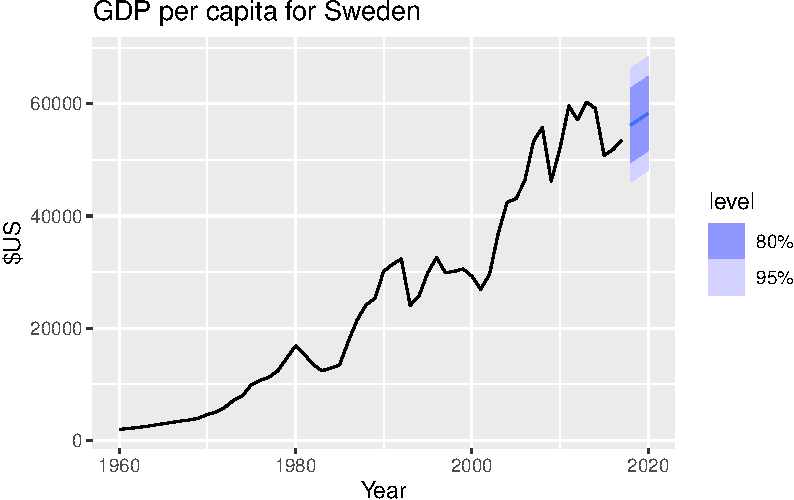
\includegraphics{chapter5_review_files/figure-pdf/unnamed-chunk-7-1.pdf}
\end{center}

Notice that the plot also contains 80\% and 95\% confidence levels (or
intervals) for your forecasts, as represented by the dark blue and light
blue ranges, respectively.

\section{Mean method}\label{mean-method}

The mean method of forecasting simply produces forecasts for future
periods that are equal to the mean of the time series considered.

\phantomsection\label{annotated-cell-8}%
\begin{Shaded}
\begin{Highlighting}[]
\NormalTok{recent\_prod }\OtherTok{\textless{}{-}} \FunctionTok{filter\_index}\NormalTok{(aus\_production, }\StringTok{"1970 Q1"} \SpecialCharTok{\textasciitilde{}} \StringTok{"2004 Q4"}\NormalTok{)}
\NormalTok{bricks }\OtherTok{\textless{}{-}}\NormalTok{ dplyr}\SpecialCharTok{::}\FunctionTok{select}\NormalTok{(recent\_prod, Bricks)}
\NormalTok{mean\_fit }\OtherTok{\textless{}{-}} \FunctionTok{model}\NormalTok{(bricks, }\FunctionTok{MEAN}\NormalTok{(Bricks)) }\hspace*{\fill}\NormalTok{\circled{1}}
\end{Highlighting}
\end{Shaded}

\begin{description}
\tightlist
\item[\circled{1}]
This is how you specify that you want to use the \texttt{MEAN()} method
for forecasting. As its argument you pass in the name of the column for
which you want to get the forecasts (\texttt{Bricks} in this case)
\end{description}

\begin{Shaded}
\begin{Highlighting}[]
\FunctionTok{tidy}\NormalTok{(mean\_fit)  }\CommentTok{\# extract output (1)}
\end{Highlighting}
\end{Shaded}

\begin{verbatim}
# A tibble: 1 x 6
  .model       term  estimate std.error statistic   p.value
  <chr>        <chr>    <dbl>     <dbl>     <dbl>     <dbl>
1 MEAN(Bricks) mean      451.      5.34      84.4 2.58e-121
\end{verbatim}

Using the \texttt{tidy()} function you can have a look at a brief report
of the mean\_fit model. You can see specifically that the estimate is
equal to the mean of the time series considered. Also, you get the
p-value which tells you about the significance of the model. Since the
p-value is very close to 0, this model is statistically significant and
we can use it to produce forecasts.

\begin{Shaded}
\begin{Highlighting}[]
\NormalTok{results\_list }\OtherTok{\textless{}{-}}\NormalTok{ mean\_fit}\SpecialCharTok{$}\StringTok{\textquotesingle{}MEAN(Bricks)\textquotesingle{}}\NormalTok{[[}\DecValTok{1}\NormalTok{]] }\CommentTok{\# extract output (2)}
\NormalTok{mean\_results }\OtherTok{\textless{}{-}}\NormalTok{ results\_list}\SpecialCharTok{$}\NormalTok{fit}

\NormalTok{mean\_fc }\OtherTok{\textless{}{-}} \FunctionTok{forecast}\NormalTok{(mean\_fit, }\AttributeTok{h =} \DecValTok{12}\NormalTok{)}
\NormalTok{bricks\_mean }\OtherTok{=} \FunctionTok{mutate}\NormalTok{(bricks,}\AttributeTok{hline=}\NormalTok{mean\_fc}\SpecialCharTok{$}\NormalTok{.mean[}\DecValTok{1}\NormalTok{]) }\CommentTok{\# add a dashed line}
\FunctionTok{autoplot}\NormalTok{(mean\_fc, bricks, }\AttributeTok{level =} \ConstantTok{NULL}\NormalTok{) }\SpecialCharTok{+}
  \FunctionTok{autolayer}\NormalTok{(bricks\_mean,hline,}\AttributeTok{linetype=}\StringTok{\textquotesingle{}dashed\textquotesingle{}}\NormalTok{,}\AttributeTok{color=}\StringTok{\textquotesingle{}blue\textquotesingle{}}\NormalTok{)}
\end{Highlighting}
\end{Shaded}

\begin{center}
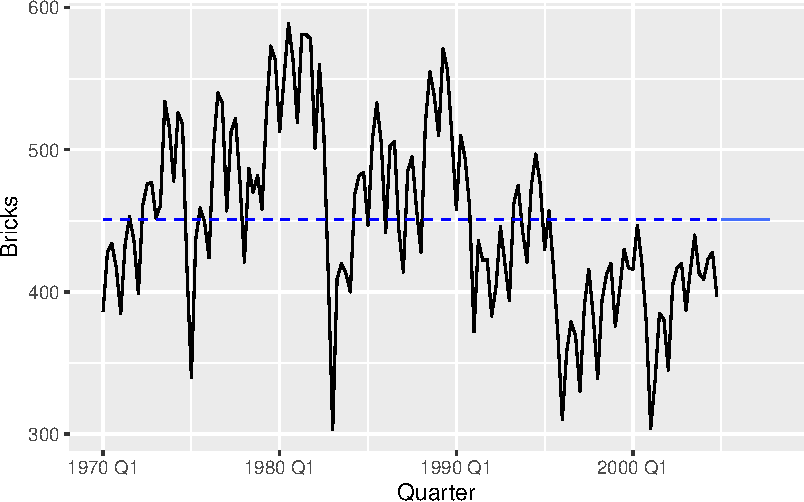
\includegraphics{chapter5_review_files/figure-pdf/unnamed-chunk-10-1.pdf}
\end{center}

The lines of code above produce the plot that shows that the forecasts
are indeed equal to the mean of the time series.

\section{Naive method}\label{naive-method}

This method produces forecasts that are just equal to the last observed
value in the time series.

\phantomsection\label{annotated-cell-11}%
\begin{Shaded}
\begin{Highlighting}[]
\NormalTok{naive\_fit }\OtherTok{\textless{}{-}} \FunctionTok{model}\NormalTok{(bricks,}\FunctionTok{NAIVE}\NormalTok{(Bricks)) }\hspace*{\fill}\NormalTok{\circled{1}}
\end{Highlighting}
\end{Shaded}

\begin{description}
\tightlist
\item[\circled{1}]
Specify the \texttt{NAIVE()} model and fit it to the data
\end{description}

\phantomsection\label{annotated-cell-12}%
\begin{Shaded}
\begin{Highlighting}[]
\NormalTok{naive\_fc }\OtherTok{\textless{}{-}} \FunctionTok{forecast}\NormalTok{(naive\_fit, }\AttributeTok{h =} \DecValTok{12}\NormalTok{) }\hspace*{\fill}\NormalTok{\circled{1}}
\end{Highlighting}
\end{Shaded}

\begin{description}
\tightlist
\item[\circled{1}]
Produce forecasts using the model specified
\end{description}

\begin{Shaded}
\begin{Highlighting}[]
\FunctionTok{autoplot}\NormalTok{(naive\_fc, bricks, }\AttributeTok{level =} \ConstantTok{NULL}\NormalTok{)}
\end{Highlighting}
\end{Shaded}

\begin{center}
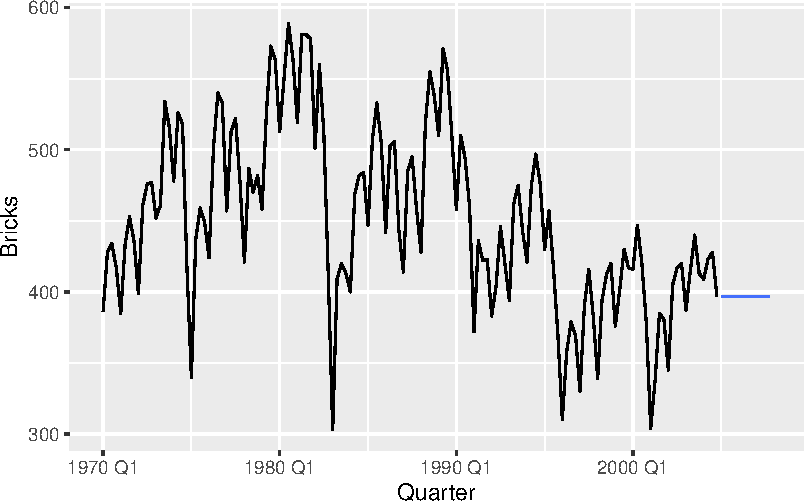
\includegraphics{chapter5_review_files/figure-pdf/unnamed-chunk-13-1.pdf}
\end{center}

The plot above just shows how the forecasts produced with this method
are equal to the last value observed in the series.

\section{Seasonal Naive}\label{seasonal-naive}

This method is similar to the Naive method but produces forecasts in the
future that are equal to the last seasonal trend observed in the data.

\phantomsection\label{annotated-cell-14}%
\begin{Shaded}
\begin{Highlighting}[]
\NormalTok{snaive\_fit }\OtherTok{\textless{}{-}} \FunctionTok{model}\NormalTok{(bricks,}\FunctionTok{SNAIVE}\NormalTok{(Bricks }\SpecialCharTok{\textasciitilde{}} \FunctionTok{lag}\NormalTok{(}\StringTok{"year"}\NormalTok{))) }\hspace*{\fill}\NormalTok{\circled{1}}
\end{Highlighting}
\end{Shaded}

\begin{description}
\tightlist
\item[\circled{1}]
specify \texttt{SNAIVE()} model indicating that the seasonal trend is
observed at a yearly interval
\end{description}

\begin{Shaded}
\begin{Highlighting}[]
\NormalTok{snaive\_fc }\OtherTok{\textless{}{-}} \FunctionTok{forecast}\NormalTok{(snaive\_fit, }\AttributeTok{h =} \DecValTok{12}\NormalTok{)}
\end{Highlighting}
\end{Shaded}

\phantomsection\label{annotated-cell-16}%
\begin{Shaded}
\begin{Highlighting}[]
\FunctionTok{autoplot}\NormalTok{(snaive\_fc, bricks, }\AttributeTok{level =} \ConstantTok{NULL}\NormalTok{) }\hspace*{\fill}\NormalTok{\circled{1}}
\end{Highlighting}
\end{Shaded}

\begin{description}
\tightlist
\item[\circled{1}]
Here the \texttt{level} argument is set to \texttt{NULL} so that the
plot does not contain forecast confidence intervals
\end{description}

\begin{center}
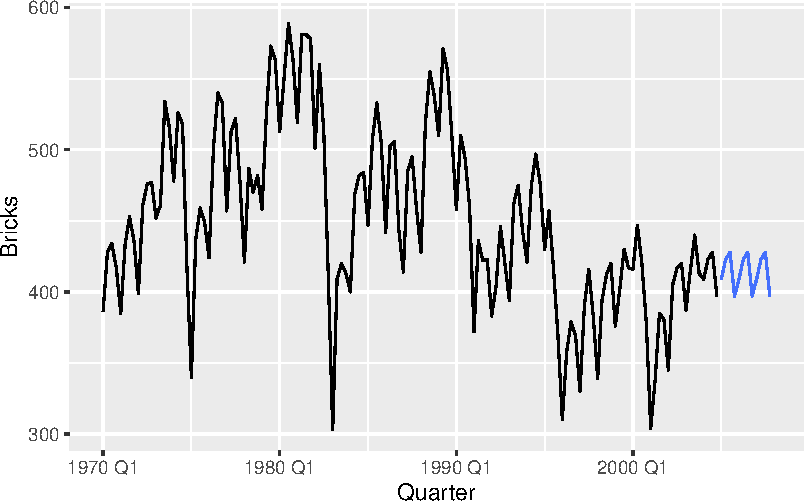
\includegraphics{chapter5_review_files/figure-pdf/unnamed-chunk-16-1.pdf}
\end{center}

\begin{Shaded}
\begin{Highlighting}[]
\NormalTok{bricks }\SpecialCharTok{\%\textgreater{}\%}
  \FunctionTok{filter\_index}\NormalTok{(}\StringTok{"Q1 2004"}\SpecialCharTok{\textasciitilde{}}\StringTok{"Q4 2004"}\NormalTok{) }\SpecialCharTok{\%\textgreater{}\%}
  \FunctionTok{autoplot}\NormalTok{()}
\end{Highlighting}
\end{Shaded}

\begin{verbatim}
Plot variable not specified, automatically selected `.vars = Bricks`
\end{verbatim}

\begin{center}
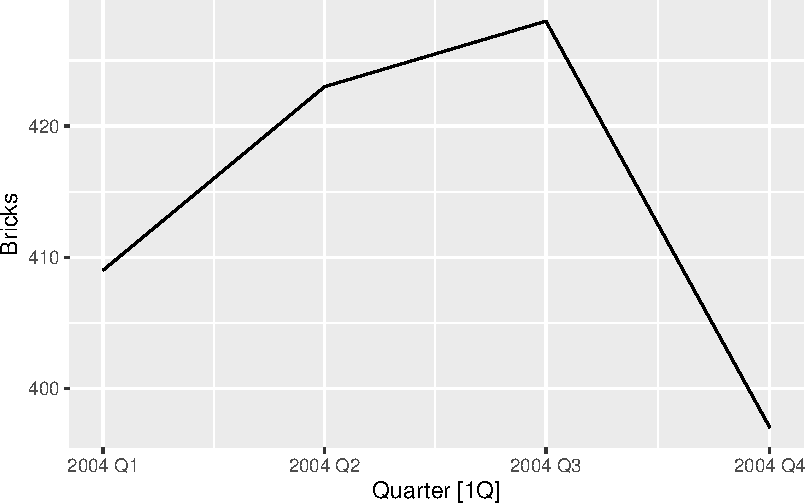
\includegraphics{chapter5_review_files/figure-pdf/unnamed-chunk-17-1.pdf}
\end{center}

Notice that the yearly trend looks something like the plot above, which
is exactly the shape that the future forecasts follow.

\section{Drift method}\label{drift-method}

This method interpolates between the first and last observation and the
line obtained is then ``stretched'' into future periods to produce
forecasts.

\begin{Shaded}
\begin{Highlighting}[]
\NormalTok{drift\_fit }\OtherTok{\textless{}{-}} \FunctionTok{model}\NormalTok{(bricks, }\FunctionTok{RW}\NormalTok{(Bricks }\SpecialCharTok{\textasciitilde{}} \FunctionTok{drift}\NormalTok{()))}
\NormalTok{drift\_fc }\OtherTok{\textless{}{-}} \FunctionTok{forecast}\NormalTok{(drift\_fit, }\AttributeTok{h =} \DecValTok{12}\NormalTok{)}
\FunctionTok{autoplot}\NormalTok{(drift\_fc, bricks, }\AttributeTok{level =} \ConstantTok{NULL}\NormalTok{)}
\end{Highlighting}
\end{Shaded}

\begin{center}
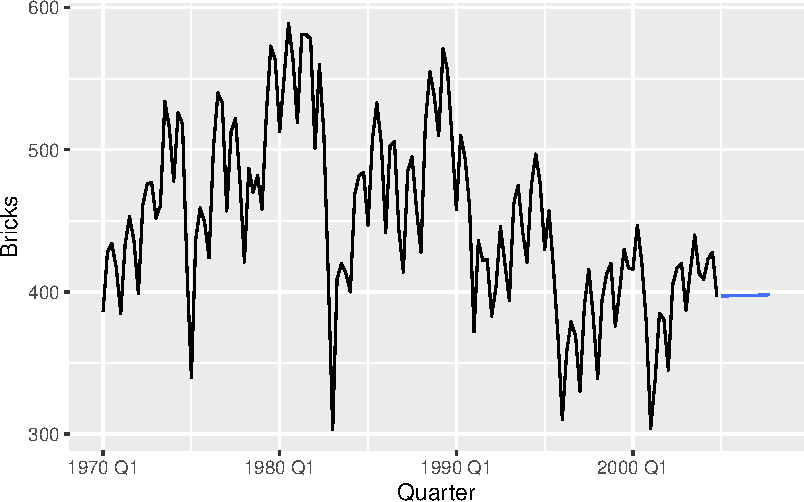
\includegraphics{chapter5_review_files/figure-pdf/unnamed-chunk-18-1.pdf}
\end{center}

To have a basic idea of how this works, we can convince ourselves that
the line used in the forecast is actually the line going from the first
to the last observation by looking at this plot.

\begin{Shaded}
\begin{Highlighting}[]
\NormalTok{T }\OtherTok{\textless{}{-}} \FunctionTok{length}\NormalTok{(bricks}\SpecialCharTok{$}\NormalTok{Bricks) }\CommentTok{\#getting length of Bricks column}
\NormalTok{b }\OtherTok{\textless{}{-}}\NormalTok{ (bricks}\SpecialCharTok{$}\NormalTok{Bricks[T] }\SpecialCharTok{{-}}\NormalTok{ bricks}\SpecialCharTok{$}\NormalTok{Bricks[}\DecValTok{1}\NormalTok{])}\SpecialCharTok{/}\NormalTok{(T }\SpecialCharTok{{-}} \DecValTok{1}\NormalTok{) }\CommentTok{\#equation of a line: slope (row140{-}row1)/(140{-}1)}
\NormalTok{a }\OtherTok{\textless{}{-}}\NormalTok{ bricks}\SpecialCharTok{$}\NormalTok{Bricks[}\DecValTok{1}\NormalTok{] }
\NormalTok{y }\OtherTok{\textless{}{-}}\NormalTok{ a }\SpecialCharTok{+}\NormalTok{ b }\SpecialCharTok{*} \FunctionTok{seq}\NormalTok{(}\DecValTok{1}\NormalTok{,T,}\AttributeTok{by=}\DecValTok{1}\NormalTok{)}

\NormalTok{DashDR }\OtherTok{\textless{}{-}} \FunctionTok{tibble}\NormalTok{(y,}\AttributeTok{Date=}\NormalTok{bricks}\SpecialCharTok{$}\NormalTok{Quarter)}
\NormalTok{DashDRts }\OtherTok{\textless{}{-}} \FunctionTok{as\_tsibble}\NormalTok{(DashDR,}\AttributeTok{index=}\NormalTok{Date)}

\FunctionTok{autoplot}\NormalTok{(drift\_fc, bricks, }\AttributeTok{level =} \ConstantTok{NULL}\NormalTok{)}\SpecialCharTok{+}
  \FunctionTok{autolayer}\NormalTok{(DashDRts,y,}\AttributeTok{color=}\StringTok{\textquotesingle{}blue\textquotesingle{}}\NormalTok{,}\AttributeTok{linetype=}\StringTok{\textquotesingle{}dashed\textquotesingle{}}\NormalTok{)}
\end{Highlighting}
\end{Shaded}

\begin{center}
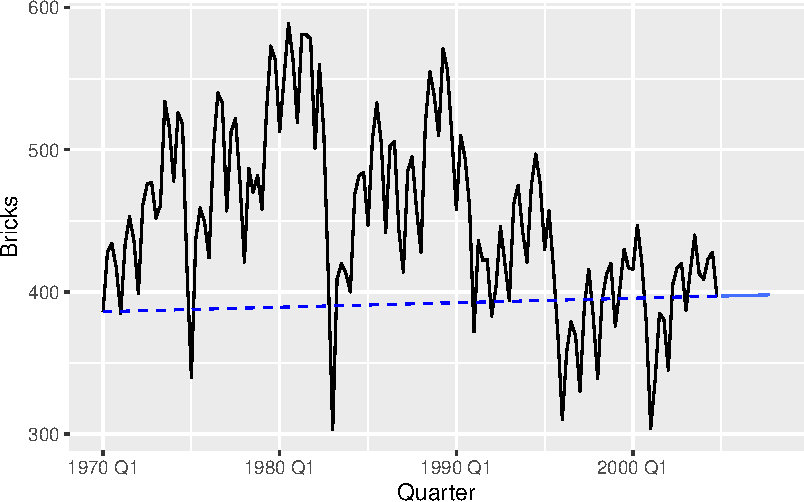
\includegraphics{chapter5_review_files/figure-pdf/unnamed-chunk-19-1.pdf}
\end{center}

Notice that T, b, a are used to compute the interpolated line and that
this follows from the equation of a line of the form \(y = mx + q\)
where \(m\) is the slope parameter (b in the code) and \(q\) is the
intercept (a in the code, which is just the first observation in the
time series).

\section{Train / Test Split}\label{train-test-split}

To test how well our model performs we need to test in on data on which
it was not trained. This is often done to prevent the problem of
\emph{overfitting} which refers to the fact that when a parameters of a
model are estimated those perform well on the data that the model has
already seen but performs poorly on new data (which is actually what
should not happen). To mitigate this problem we divide our dataset into
a \emph{train} and a \emph{test} portion.

\phantomsection\label{annotated-cell-20}%
\begin{Shaded}
\begin{Highlighting}[]
\NormalTok{train }\OtherTok{\textless{}{-}} \FunctionTok{filter\_index}\NormalTok{(aus\_production, }\StringTok{"1992 Q1"} \SpecialCharTok{\textasciitilde{}} \StringTok{"2006 Q4"}\NormalTok{) }\hspace*{\fill}\NormalTok{\circled{1}}
\end{Highlighting}
\end{Shaded}

\begin{description}
\tightlist
\item[\circled{1}]
Our train dataset is made only of observations from 1992 to 2006.
\end{description}

\phantomsection\label{annotated-cell-21}%
\begin{Shaded}
\begin{Highlighting}[]
\NormalTok{beer\_fit }\OtherTok{\textless{}{-}} \FunctionTok{model}\NormalTok{(train, }\AttributeTok{Mean =} \FunctionTok{MEAN}\NormalTok{(Beer), }\AttributeTok{Naive =} \FunctionTok{NAIVE}\NormalTok{(Beer),}
\StringTok{\textquotesingle{}Seasonal naive\textquotesingle{}} \OtherTok{=} \FunctionTok{SNAIVE}\NormalTok{(Beer)) }\hspace*{\fill}\NormalTok{\circled{1}}
\NormalTok{beer\_fc }\OtherTok{\textless{}{-}} \FunctionTok{forecast}\NormalTok{(beer\_fit, }\AttributeTok{h =} \DecValTok{14}\NormalTok{) }\hspace*{\fill}\NormalTok{\circled{2}}
\end{Highlighting}
\end{Shaded}

\begin{description}
\tightlist
\item[\circled{1}]
fit three different models using the MEAN, NAIVE, and SNAIVE methods
\item[\circled{2}]
produce forecasts based on these three models
\end{description}

\begin{Shaded}
\begin{Highlighting}[]
\FunctionTok{autoplot}\NormalTok{(beer\_fc, train, }\AttributeTok{level =} \ConstantTok{NULL}\NormalTok{) }\SpecialCharTok{+}
  \FunctionTok{autolayer}\NormalTok{(}\FunctionTok{filter\_index}\NormalTok{(aus\_production, }\StringTok{"2007 Q1"} \SpecialCharTok{\textasciitilde{}}\NormalTok{ .),}
  \AttributeTok{colour =} \StringTok{"black"}\NormalTok{) }\SpecialCharTok{+} \FunctionTok{labs}\NormalTok{(}\AttributeTok{y =} \StringTok{"Megalitres"}\NormalTok{, }\AttributeTok{title =} \StringTok{"Forecasts}
\StringTok{            for quarterly beer production"}\NormalTok{) }\SpecialCharTok{+}
  \FunctionTok{guides}\NormalTok{(}\AttributeTok{colour =} \FunctionTok{guide\_legend}\NormalTok{(}\AttributeTok{title =} \StringTok{"Forecast"}\NormalTok{))}
\end{Highlighting}
\end{Shaded}

\begin{verbatim}
Plot variable not specified, automatically selected `.vars = Beer`
\end{verbatim}

\begin{center}
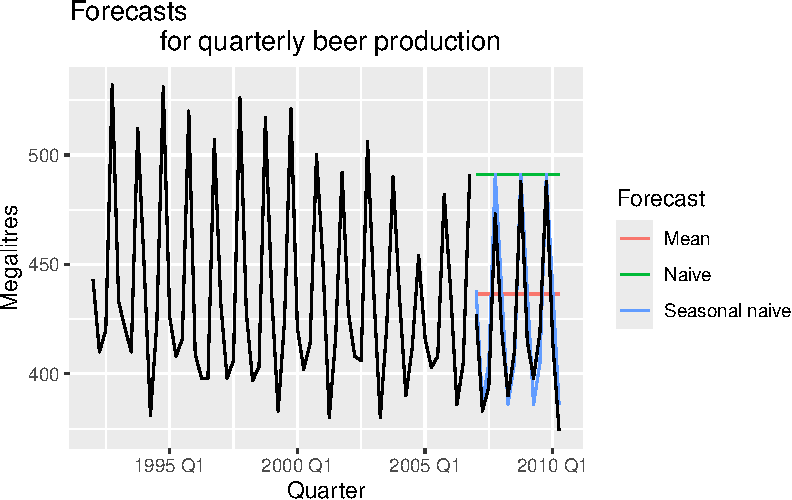
\includegraphics{chapter5_review_files/figure-pdf/unnamed-chunk-22-1.pdf}
\end{center}

Now we can plot how well the three different models perform and we can
see that the Seasonal Naive produces more accurate forecasts as it is
closer to the original series (black line). Notice, that by the way they
were constructed, the models did not see all the data in the series but
they were trained only on data up to 2006. Nonetheless, the Seasonal
Naive performs pretty well when it tries to make forecasts on data it
did not see.




\end{document}
